
\documentclass[a4paper,final,12pt]{article}
%%%%%%%%%%%%%%%%%%%%%%%%%%%%%%%%%%%%%%%%%%%%%%%%%%%%%%%%%%%%%%%%%%%%%%%%%%%%%%%%%%%%%%%%%%%%%%%%%%%%%%%%%%%%%%%%%%%%%%%%%%%%%%%%%%%%%%%%%%%%%%%%%%%%%%%%%%%%%%%%%%%%%%%%%%%%%%%%%%%%%%%%%%%%%%%%%%%%%%%%%%%%%%%%%%%%%%%%%%%%%%%%%%%%%%%%%%%%%%%%%%%%%%%%%%%%
\usepackage{graphicx,hyperref,mathpple,amsmath,exscale,setspace,xcolor}
\usepackage[left=20mm,right=20mm,top=20mm,bottom=20mm]{geometry}
\usepackage{pdflscape,showkeys,changepage}
\usepackage[TABBOTCAP]{subfigure}
\usepackage[round]{natbib}

\setcounter{MaxMatrixCols}{10}
%TCIDATA{OutputFilter=LATEX.DLL}
%TCIDATA{Version=5.50.0.2953}
%TCIDATA{<META NAME="SaveForMode" CONTENT="2">}
%TCIDATA{BibliographyScheme=BibTeX}
%TCIDATA{Created=Wednesday, May 03, 2023 13:45:06}
%TCIDATA{LastRevised=Thursday, February 29, 2024 14:04:57}
%TCIDATA{<META NAME="GraphicsSave" CONTENT="32">}
%TCIDATA{<META NAME="DocumentShell" CONTENT="Standard LaTeX\Blank - Standard LaTeX Article">}
%TCIDATA{CSTFile=40 LaTeX article.cst}

\AtBeginDocument{
\let\oldref\ref\renewcommand{\ref}[1]{(\oldref{#1})}
\newcommand{\bsq}{\begin{subequations}}\newcommand{\esq}{\end{subequations}}
\newcommand{\bls}{\begin{landscape}}\newcommand{\els}{\end{landscape}}
\renewcommand\showkeyslabelformat[1]{{\parbox[t]{\marginparwidth}{\raggedright\footnotesize\url{#1}}}}
\newcommand{\intxt}[1]{\intertext{#1}}\newcommand{\BAW}[1]{\begin{adjustwidth}{-#1mm}{-5mm}}\newcommand{\EAW}{\end{adjustwidth}}
\newcommand{\vsp}[1]{\vspace*{#1mm}}\newcommand{\hsp}[1]{\hspace*{#1mm}}  }
\renewcommand\section{\@startsection{section}{1}{\z@}{-2.5ex \@plus -1ex \@minus -.2ex}{0.01ex \@plus.2ex}{\Large\bfseries}}
\renewcommand\subsection{\@startsection{subsection}{1}{\z@}{-1.5ex \@plus -1ex \@minus -.2ex}{0.01ex \@plus.2ex}{\large\bfseries}}
\makeatletter
\renewcommand*{\@fnsymbol}[1]{\ensuremath{\ifcase#1\or *\or
    \#\or \star\or \bowtie\or \star\star\or \ddagger\ddagger \else\@ctrerr\fi}}
\makeatother
\allowdisplaybreaks
\IfFileExists{C:/swp55/TCITeX/TeX/LaTeX/SWmacros/tcilatex.tex}{\input{tcilatex}}{}
\graphicspath{{./graphics/}{../graphics/}{../../graphics/}{../../../graphics/}}
\definecolor{myred}{rgb}{.50,.10,.10}
\definecolor{mygrn}{rgb}{.10,.35,.10}
\definecolor{myblu}{rgb}{.10,.10,.35}
\hypersetup{colorlinks,citecolor=myblu,filecolor=mygrn,linkcolor=myred,urlcolor=mygrn,breaklinks=true}
\setstretch{1.2345}
\setlength{\parskip}{7pt}

\begin{document}


\section{HP97}

The Hodrick and Prescott (1997, HP) Filter can be expressed in State Space
Form (SSF)\ using the following Unobserved Component (UC)\ model structure:%
\bsq\label{HP0}%
\begin{align}
y_{t}& =y_{t}^{\ast }+y_{t}^{c}  \label{HP0a} \\
\Delta ^{2}y_{t}^{\ast }& =\varepsilon _{1t}  \label{HP0b} \\
y_{t}^{c}& =\psi \varepsilon _{2t},  \label{HP0c}
\end{align}%
\esq where $y_{t}$ is (100 times) the log of GDP, and the shocks $\left\{
\varepsilon _{it}\right\} _{i=1}^{2}$ are mutually uncorrelated $i.i.d.$ $%
N(0,1)$. The standard deviation $\psi $ is the (square root of the)
smoothing parameter, commonly set to $40$ for quarterly macroeconomic data,
implying a value of `$\lambda $' of $1600$.

The `\emph{numbered} \emph{shock}' to `\emph{named shock}' mapping is:%
\begin{equation}
\begin{bmatrix}
\varepsilon _{1t} \\ 
\varepsilon _{2t}%
\end{bmatrix}%
=%
\begin{bmatrix}
\varepsilon _{t}^{\ast } \\ 
\varepsilon _{t}^{c}%
\end{bmatrix}%
,
\end{equation}%
where $\varepsilon _{t}^{\ast }$ is the trend (or permanent)\ shock and $%
\varepsilon _{t}^{c}$ is the cycle (or transitory) shock.

\section{Shock recovery}

\subsection{State Space Models with lagged states}

Kurz (2018) adopts the following general SSF\ with lagged states in the
measurement:\bsq\label{SSM}%
\begin{align}
\mathsf{Measurement}& :\quad Z_{t}=D_{1}X_{t}+D_{2}X_{t-1}+R\varepsilon _{t}
\label{ssm1} \\
\mathsf{State}& :\quad X_{t}=\Phi X_{t-1}+Q\varepsilon _{t},  \label{ssm2}
\end{align}%
\esq where $\varepsilon _{t}\sim MN(0_{m},I_{m})$, $D_{1},D_{2},\Phi ,R$ are 
$Q$ are conformable system matrices, $Z_{t}$ the observed variable and $X_{t}
$ the latent state variable, and $m$ is the number of shocks $\left\{
\varepsilon _{it}\right\} _{i=1}^{2}$.

\subsection{HP97 in `\emph{shock recovery}' SSF}

To assess shock recovery, write the model in \ref{HP0} in `\emph{shock
recovery}' SSF by collecting all observable variables in $Z_{t}$ and all
shocks (and other latent state variables)\ in $X_{t}$. Differencing $y_{t}$
and $y_{t}^{c}$ twice, and re-arranging the relations in \ref{HP0} then
yields:%
\begin{align}
\Delta ^{2}y_{t}& =\Delta ^{2}y_{t}^{\ast }+\Delta ^{2}y_{t}^{c}  \notag \\
& =\varepsilon _{1t}+\psi \Delta ^{2}\varepsilon _{2t}  \notag \\
& =\varepsilon _{1t}+\psi \varepsilon _{2t}-2\psi \varepsilon _{2t-1}+\psi
\varepsilon _{2t-2},  \label{Z}
\end{align}%
where $\Delta ^{2}y_{t}$ is the only observed variable.

The Measurement and State equations of the `\emph{shock recovery}' SSF
corresponding to the relations in \ref{Z} are then given by:\bsq\label{K0SSM}%
\begin{align}
\mathsf{Measurement}:\quad Z_{t}& =D_{1}X_{t}+D_{2}X_{t-1}+R\varepsilon _{t}
\notag \\
\Leftrightarrow \Delta ^{2}y_{t}& =\varepsilon _{1t}+\psi \varepsilon
_{2t}-2\psi \varepsilon _{2t-1}+\psi \varepsilon _{2t-2} \\[2mm]
Z_{t}& =\underbrace{%
\begin{bmatrix}
1 & \psi  & 0%
\end{bmatrix}%
}_{D_{1}}\underbrace{%
\begin{bmatrix}
\varepsilon _{1t} \\ 
\varepsilon _{2t} \\ 
\varepsilon _{2t-1}%
\end{bmatrix}%
}_{X_{t}}+\underbrace{%
\begin{bmatrix}
0 & -2\psi  & \psi 
\end{bmatrix}%
}_{D_{2}}\underbrace{%
\begin{bmatrix}
\varepsilon _{1t-1} \\ 
\varepsilon _{2t-1} \\ 
\varepsilon _{2t-2}%
\end{bmatrix}%
}_{X_{t-1}}+\underbrace{%
\begin{bmatrix}
0 & 0%
\end{bmatrix}%
}_{R}\underbrace{%
\begin{bmatrix}
\varepsilon _{1t} \\ 
\varepsilon _{2t}%
\end{bmatrix}%
}_{\varepsilon _{t}} \\
\mathsf{State}:\quad X_{t}& =\Phi X_{t-1}+Q\varepsilon _{t},  \notag \\[5mm]
\underbrace{%
\begin{bmatrix}
\varepsilon _{1t} \\ 
\varepsilon _{2t} \\ 
\varepsilon _{2t-1}%
\end{bmatrix}%
}_{X_{t}}& =\underbrace{%
\begin{bmatrix}
0 & 0 & 0 \\ 
0 & 0 & 0 \\ 
0 & 1 & 0%
\end{bmatrix}%
}_{\Phi }\underbrace{%
\begin{bmatrix}
\varepsilon _{1t-1} \\ 
\varepsilon _{2t-1} \\ 
\varepsilon _{2t-2}%
\end{bmatrix}%
}_{X_{t-1}}+\underbrace{%
\begin{bmatrix}
1 & 0 \\ 
0 & 1 \\ 
0 & 0%
\end{bmatrix}%
}_{Q}\underbrace{%
\begin{bmatrix}
\varepsilon _{1t} \\ 
\varepsilon _{2t}%
\end{bmatrix}%
}_{\varepsilon _{t}}.
\end{align}%
\esq

\subsection{Shock recovery}

The diagonal entries of the steady-state variance/covariance matrix of the
smoothed and filtered states $X_{t}$ denoted by $P_{t|T}^{\ast }$ and $%
P_{t|t}^{\ast }$, respectively, are:%
\begin{equation}
\begin{tabular}{ccccc}
\hline
Shocks &  & $\mathrm{diag}(P_{t|T}^{\ast })$ &  & $\mathrm{diag}%
(P_{t|t}^{\ast })$ \\ \hline
{$\varepsilon _{1t}$} &  & $0.9439$ &  & $0.9995$ \\ 
{$\varepsilon _{2t}$} &  & $0.0561$ &  & $0.2006$ \\ \hline
\end{tabular}%
~,  \label{Pstar}
\end{equation}%
indicating that the trend (or permanent) shock $\varepsilon
_{1t}=\varepsilon _{t}^{\ast }$ cannot be recovered ($P^{\ast }\approx 1$),
while the cycle shock $\varepsilon _{2t}=\varepsilon _{t}^{c}$ appears to be
recoverable ($P^{\ast }\approx 0$). In \autoref{fig:1}, simulated states and
estimated Kalman smoothed states are plotted for the two shocks of interest.

\begin{figure}[h!]
\centering
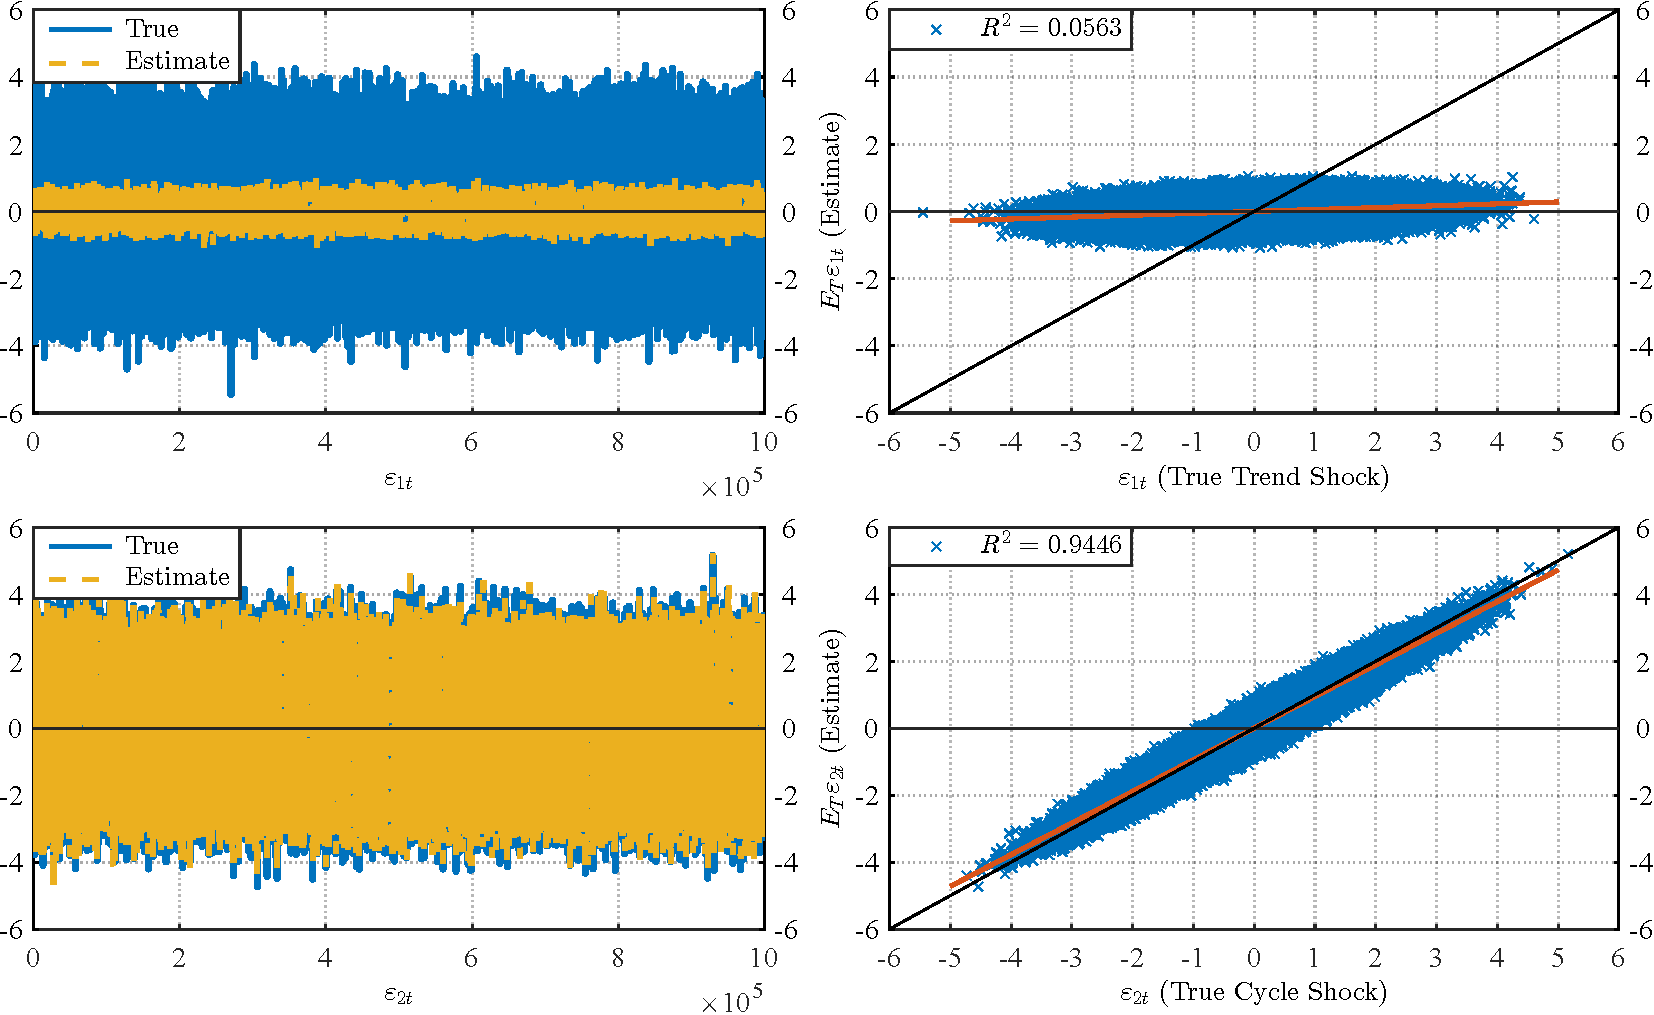
\includegraphics[width=1\textwidth,trim={0 0 0
0},clip,angle=00]{HP97_plots_KS.pdf}
\caption{Comparison of true shocks and Kalman Smoothed estimates $\protect%
\varepsilon _{t|T}$.}
\label{fig:1}
\end{figure}
The correlation between the true (simulated) and estimated Kalman smoothed
shocks can be analyzed by simply computing $\mathrm{Corr}(X_{t},\hat{X}%
_{t|T})$, where $X_{t}=%
\begin{bmatrix}
\varepsilon _{1t} & \varepsilon _{2t} & \varepsilon _{2t-1}%
\end{bmatrix}%
^{\prime }$ and $\hat{X}_{t|T}=E_{T}X_{t}=E_{T}%
\begin{bmatrix}
\varepsilon _{1t} & \varepsilon _{2t} & \varepsilon _{2t-1}%
\end{bmatrix}%
^{\prime }$, yielding (for the first two elements of $X_{t}$):%
\begin{equation}
\begin{tabular}{ccc}
\hline
Shocks &  & $\mathrm{Corr}(X_{t},\hat{X}_{t|T})$ \\ \hline
$\varepsilon _{1t}$ &  & $0.2368$ \\ 
$\varepsilon _{2t}$ &  & $0.9713$ \\ \hline
\end{tabular}%
~.  \label{Corr}
\end{equation}%
As can be seen from \ref{Corr}, the estimated permanent shock $\varepsilon
_{1t}$ is only weakly correlated ($0.2368$) with the true value. The
estimated cyclical shock $\varepsilon _{2t}$, on the other hand, is highly
correlated ($0.9713$) with the true value.\ These facts can also be seen
from \autoref{fig:1} below.

\subsection{Shock Identities}

Kalman Filter estimates of the permanent and transitory shocks $\varepsilon
_{1t}$ and $\varepsilon _{2t}$ are linked by the identity:%
\begin{equation}
E_{t}\varepsilon _{2t}=\psi E_{t}\varepsilon _{1t},  \label{KF}
\end{equation}%
and the corresponding Kalman Smoother estimates are linked by the \emph{%
dynamic} identity: 
\begin{equation}
\Delta ^{2}E_{T}\varepsilon _{1t}=\frac{1}{\psi }E_{T}\varepsilon _{2t-2}.
\label{KS}
\end{equation}%
The filtered and smoothed estimates of the contemporaneous correlations are,
respectively: 
\begin{equation*}
\begin{tabular}{ccc}
\multicolumn{3}{c}{$\mathrm{Corr}(\hat{X}_{t|t},\hat{X}_{t|t})$} \\ \hline
Shocks & {$\varepsilon _{1t}$} & {$\varepsilon _{2t}$} \\ \hline
{$\varepsilon _{1t}$} & \multicolumn{1}{r}{$\phantom{-}1.0000$} & 
\multicolumn{1}{r}{$\phantom{-}1.0000$} \\ 
{$\varepsilon _{2t}$} & \multicolumn{1}{r}{$1.0000$} & \multicolumn{1}{r}{$%
1.0000$} \\ \hline
\end{tabular}%
\text{ \ \ \ \ \ \ \ and \ \ \ \ \ \ \ }%
\begin{tabular}{ccc}
\multicolumn{3}{c}{$\mathrm{Corr}(\hat{X}_{t|T},\hat{X}_{t|T})$} \\ \hline
Shocks & {$\varepsilon _{1t}$} & {$\varepsilon _{2t}$} \\ \hline
{$\varepsilon _{1t}$} & \multicolumn{1}{r}{$1.0000$} & \multicolumn{1}{r}{$%
-0.1907$} \\ 
{$\varepsilon _{2t}$} & \multicolumn{1}{r}{$-0.1907$} & \multicolumn{1}{r}{$%
1.0000$} \\ \hline
\end{tabular}%
~\text{.}
\end{equation*}%
Note that {$\varepsilon _{1t}$ and $\varepsilon _{2t}$ }were generated as $%
i.i.d.$ $N(0,1)$ and mutually uncorrelated.

Running regressions corresponding to \ref{KF} and \ref{KS} obtained from the
simulated data (without an intercept) yields regression coefficient of $40$
and $0.025=1/40$ when the smoothing parameter was set to $\lambda
=1600=40^{2}$ in the simulation. The regression fit is perfect, yielding an $%
R^{2}$ of $1$ and a residual sum of squares of exactly $0$ (see Panels (a)
and (b) in \autoref{tab:KF}, respectively). The file \texttt{HP97.m}
replicates the output summarized here.

% \begin{table}[h!]
% \subfigure[Kalman Filter]   {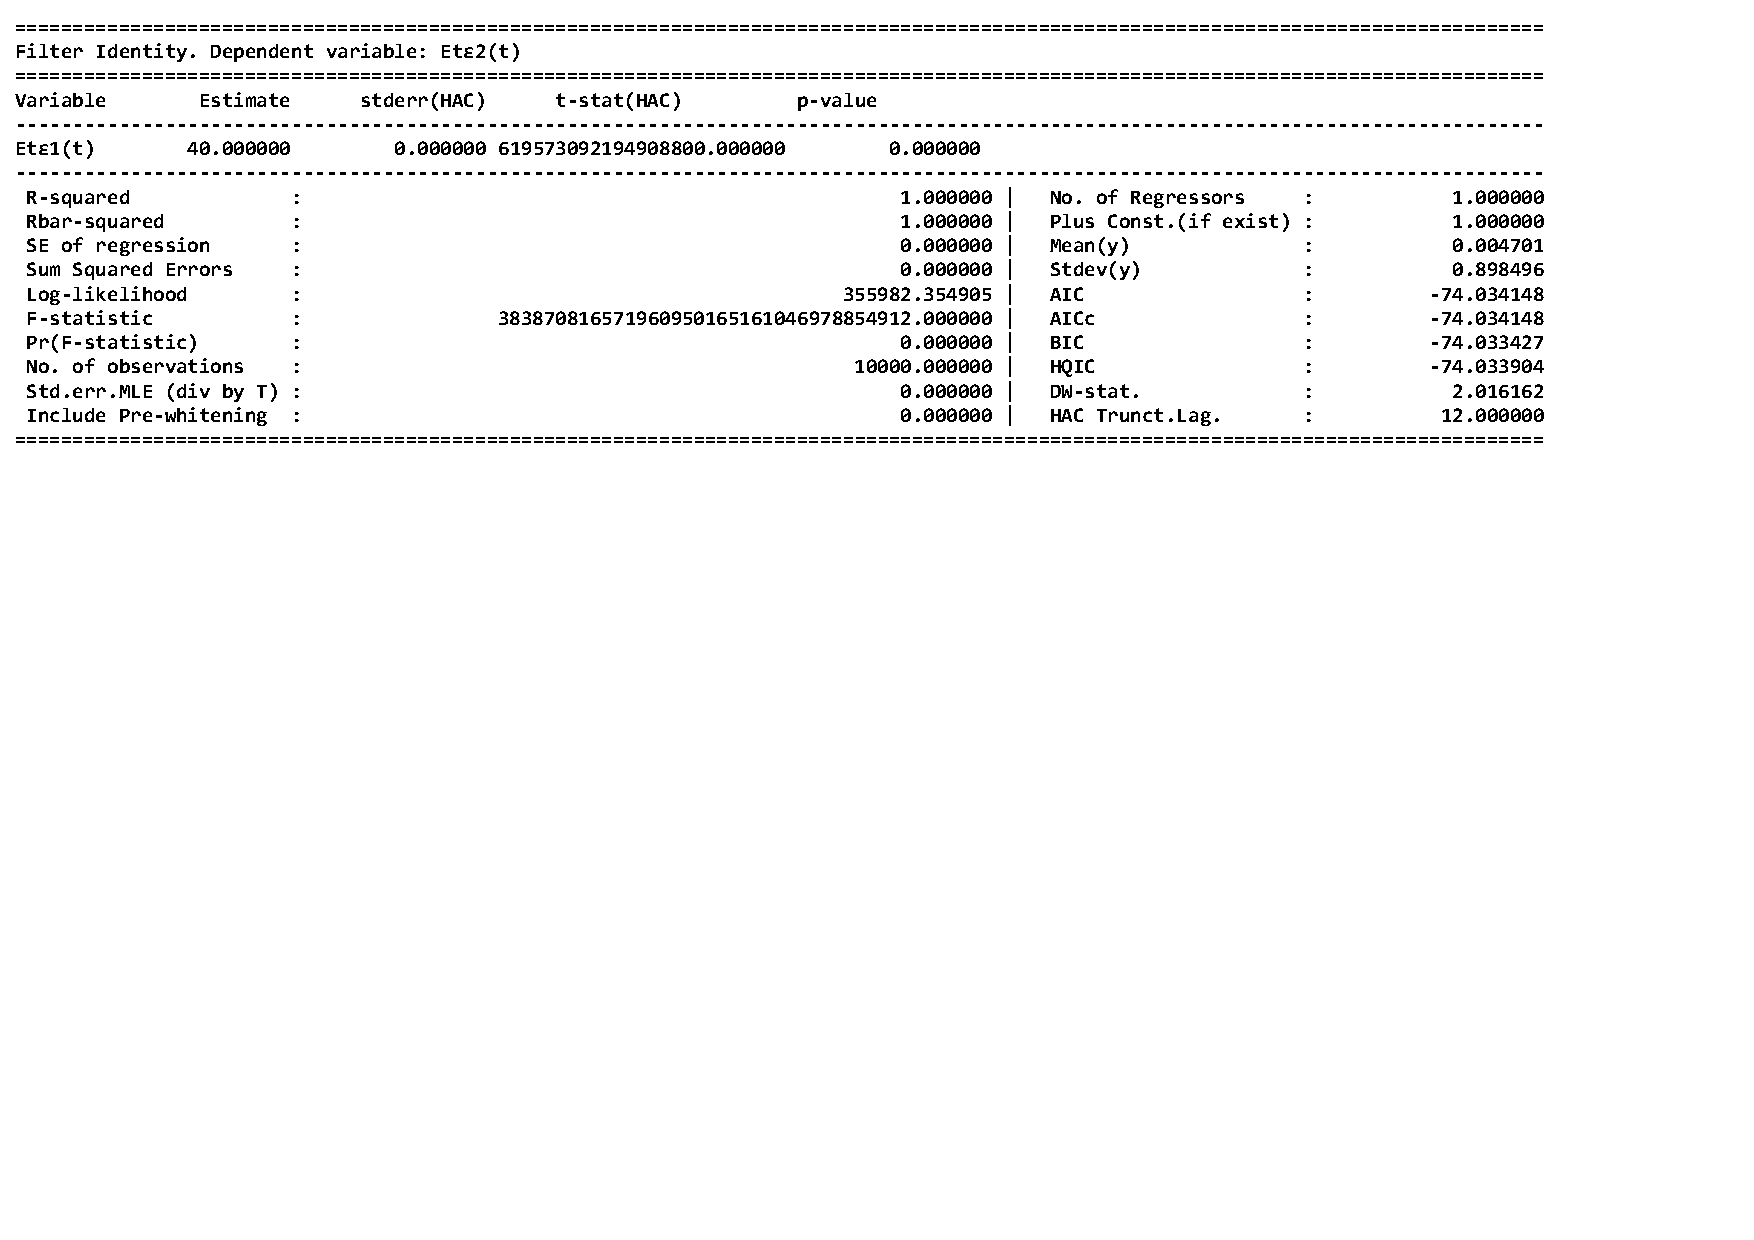
\includegraphics[width=\textwidth]{hp_filter}} %
% \subfigure[Kalman Smoother] {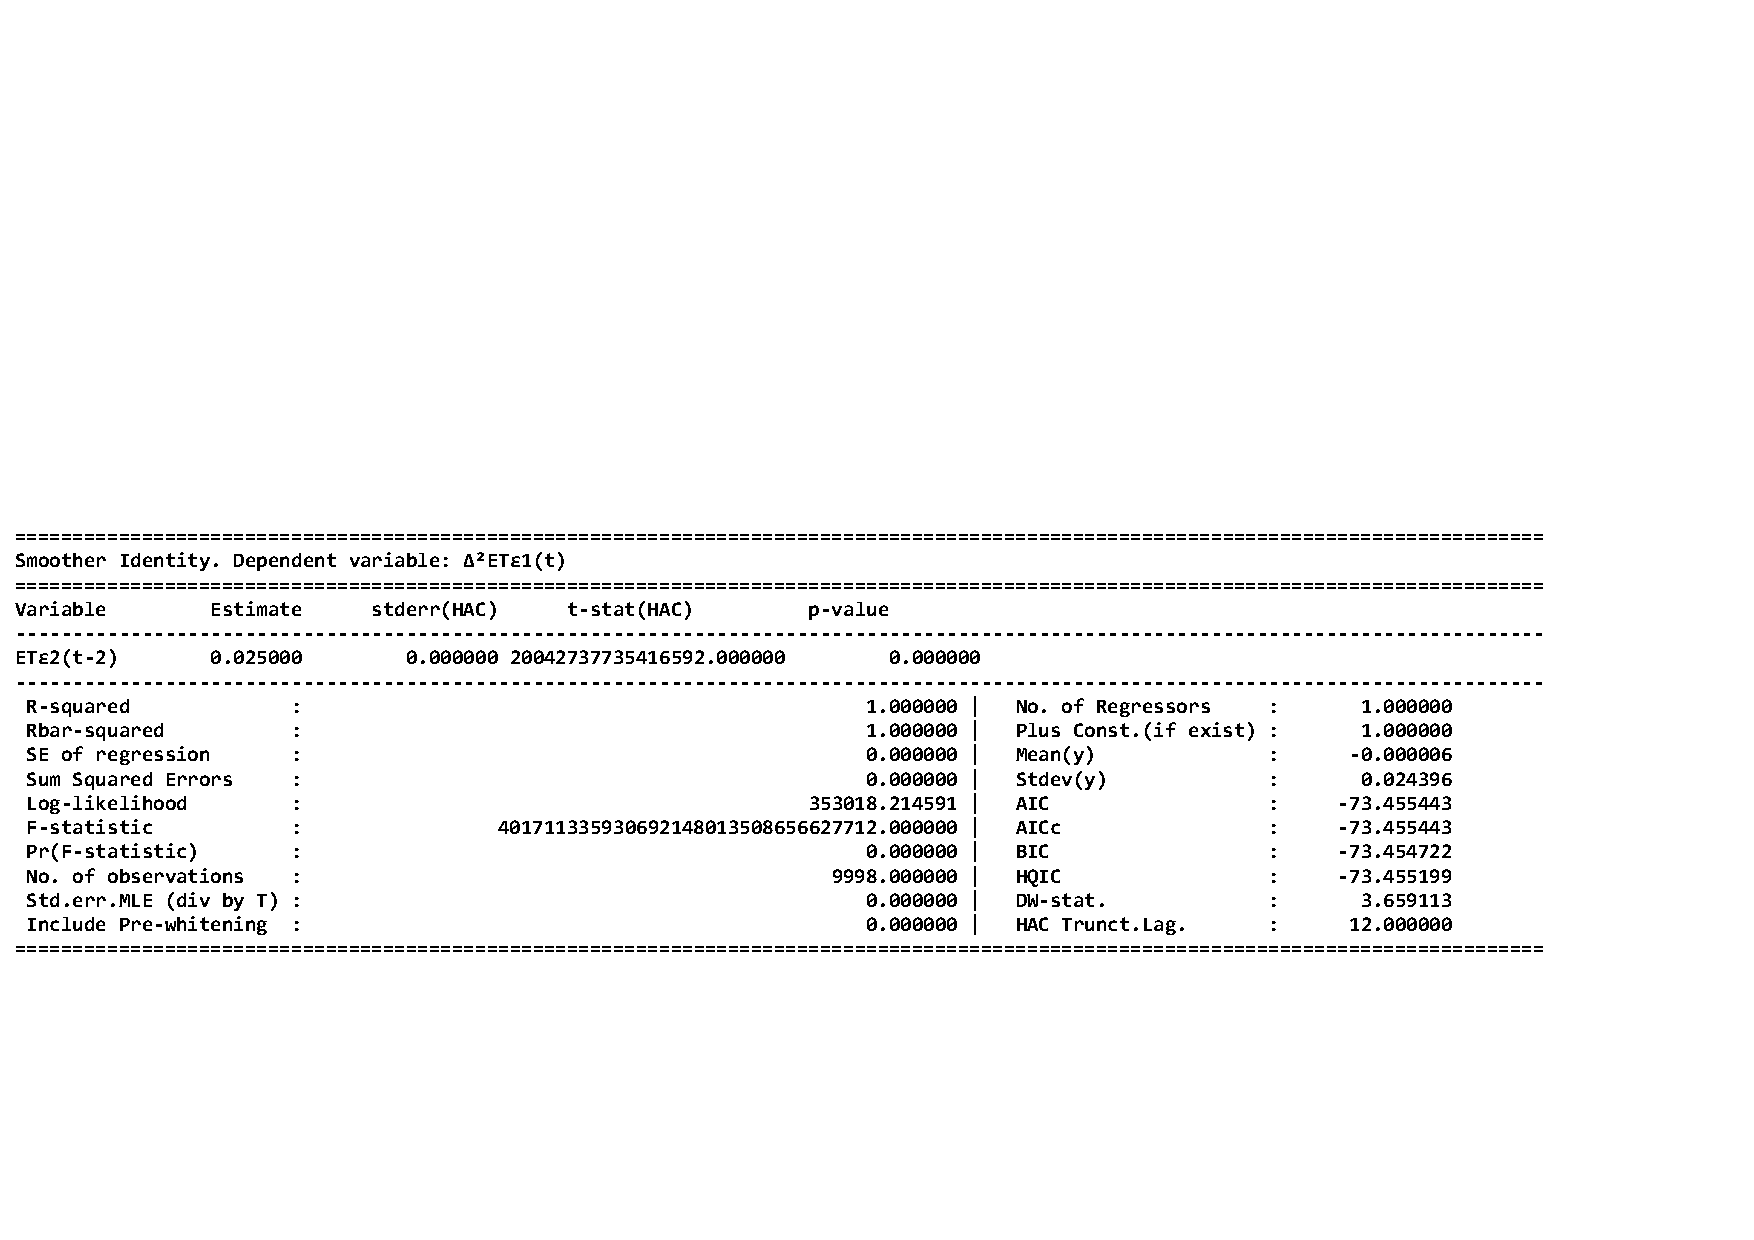
\includegraphics[width=\textwidth]{hp_smoother}}
% \vspace{-3mm}
% \caption{Shock identity regressions using Kalman filter and smoother
% estimates.}
% \label{tab:KF}
% \end{table}

\begin{table}[h!]
  \subfigure[Kalman Filter]   {\includegraphics[width=\textwidth]{HP_filter_a}} %
  \subfigure[Kalman Smoother] {\includegraphics[width=\textwidth]{HP_filter_b}}
  \vspace{-3mm}
  \caption{Shock identity regressions using Kalman filter and smoother
  estimates.}
  \label{tab:KF}
  \end{table}

Since $\varepsilon _{1t}=\Delta ^{2}y_{t}^{\ast }$ and $\varepsilon _{2t}=%
\frac{1}{\psi }y_{t}^{c}$, this implies that the output from the standard
HP--Filter will give the corresponding idenity to \ref{KS} as:%
\begin{alignat}{2}
& & \Delta ^{2}\underbrace{E_{T}\varepsilon _{1t}}_{\Delta ^{2}y_{t}^{\ast
}}& =\frac{1}{\psi }\underbrace{E_{T}\varepsilon _{2t-2}}_{\frac{1}{\psi }%
y_{t-2}^{c}}  \notag \\
& \Leftrightarrow & \Delta ^{4}y_{t}^{\ast }& =\frac{1}{\psi ^{2}}%
y_{t-2}^{c},  \notag \\
& \Leftrightarrow ~~~ & \Delta ^{4}\text{HP--trend}_{t}& =\frac{1}{\psi ^{2}}%
\text{HP--cycle}_{t-2},  \notag
\end{alignat}%
so that a regression of the fourth differenced HP--trend on a twice lagged
HP--cycle will give a coefficient estimate of $\frac{1}{40^{2}}=\frac{1}{1600%
}=0.000625$. The HP-Filter appears to be able to recover the transitory
cyclical shock $\varepsilon _{2t}=\varepsilon _{t}^{c}$, but not the
permanent shock. HP-Filter estimates of $\varepsilon _{1t}$ and $\varepsilon
_{2t}$ induce a negative correlation between trend-cycle shocks, ie., $%
\mathrm{Corr}(E_{T}\varepsilon _{1t},E_{T}\varepsilon _{2t})=-0.1907$,
despite being generated with zero correlation.

\bigskip

\bigskip

\bigskip

\bigskip

\bigskip

\bigskip

\bigskip

\bigskip

\bigskip

\bigskip

\bigskip

\bigskip

\bigskip

\bigskip

\end{document}
